% !TEX program = xelatex
\documentclass[14pt,aspectratio=169]{beamer}

\usepackage[english, russian]{babel}
\usepackage{fontspec}
\usepackage{unicode-math}

% Настройка шрифтов с fallback
\setmainfont{Times New Roman}[
    Ligatures=TeX,
    Numbers=OldStyle
]
\setsansfont{Liberation Sans}[
    Ligatures=TeX
]

% Дополнительные пакеты для улучшения отображения
\usepackage{graphicx}
\usepackage{amsmath}
\usepackage{amsfonts}
\usepackage{amssymb}
\usepackage{mathtools}

\usetheme{Madrid}
\usecolortheme{default}

% Улучшение отображения математики
\usefonttheme{serif}

% Настройки для русского языка (для новых версий babel)
% Если используется старая версия, эти строки можно закомментировать

% Улучшение отображения текста
\setbeamertemplate{navigation symbols}{}
\setbeamertemplate{footline}[frame number]

% Настройка отступов и интервалов
\setlength{\parskip}{0.5em}

% Улучшение отображения списков
\setbeamertemplate{itemize item}{\raisebox{0.12ex}{\scriptsize$\bullet$}}
\setbeamertemplate{itemize subitem}{\raisebox{0.12ex}{\tiny$\bullet$}}

% Улучшение отображения блоков
\setbeamertemplate{blocks}[rounded][shadow=true]

\title{Стабилизация неполноприводной системы Segway \\ методом управления по выходу}
\author{Зыкин Л. В. \\ Группа R3435}
\institute{Университет ИТМО \\ Факультет систем управления и робототехники}
\date{}

\begin{document}

\frame{\titlepage}

\begin{frame}
\frametitle{Содержание}
\tableofcontents
\end{frame}

\section{Введение}

\section{Описание системы Segway}

\begin{frame}
\frametitle{Физическая модель}
\begin{columns}
\column{0.5\textwidth}
\begin{itemize}
    \item Двухколесное транспортное средство
    \item Платформа с маятником
    \item Два независимых колеса
    \item Одно управляющее воздействие
\end{itemize}

\column{0.5\textwidth}
\begin{block}{Параметры}
\begin{itemize}
    \item $M = 10$ кг
    \item $m = 2$ кг
    \item $L = 0.5$ м
    \item $R = 0.1$ м
\end{itemize}
\end{block}
\end{columns}
\end{frame}

\begin{frame}
\frametitle{Математическая модель}
\begin{block}{Вектор состояния}
\[
\mathbf{x} = \begin{bmatrix} \theta & \dot{\theta} & \phi & \dot{\phi} & x & \dot{x} \end{bmatrix}^T
\]
\end{block}

\begin{block}{Уравнения движения}
\[
\mathbf{M}(\theta) \begin{bmatrix} \ddot{\theta} \\ \ddot{\phi} \end{bmatrix} + \mathbf{C}(\theta, \dot{\phi}) + \mathbf{G}(\theta) = \begin{bmatrix} u \\ -u \end{bmatrix}
\]
\end{block}

\begin{block}{Свойство неполноприводности}
Число степеней свободы: $n = 2$ \\
Число управлений: $m = 1$ \\
Условие: $m < n$
\end{block}
\end{frame}

\section{Задача управления}

\begin{frame}
\frametitle{Постановка задачи стабилизации}
\begin{block}{Цель управления}
\[
\lim_{t \to \infty} \theta(t) = 0, \quad \lim_{t \to \infty} \dot{\theta}(t) = 0
\]
\end{block}

\begin{block}{Требования}
\begin{itemize}
    \item Ограниченность управления: $|u(t)| \leq u_{\max}$
    \item Минимизация времени установления
    \item Минимизация перерегулирования
    \item Обеспечение устойчивости
\end{itemize}
\end{block}
\end{frame}

\begin{frame}
\frametitle{Метод управления по выходу}
\begin{block}{Выходные переменные}
\[
\mathbf{y} = \begin{bmatrix} \theta & \dot{\theta} \end{bmatrix}^T
\]
Измеряются с помощью IMU (гироскоп + акселерометр)
\end{block}

\begin{block}{Закон управления}
\[
u = -K_p \theta - K_d \dot{\theta}
\]
ПД-регулятор по выходу
\end{block}

\begin{block}{Преимущества}
\begin{itemize}
    \item Использует только измеряемые переменные
    \item Простота реализации
    \item Низкая стоимость датчиков
\end{itemize}
\end{block}
\end{frame}

\section{Моделирование свободного движения}

\begin{frame}
\frametitle{Результаты моделирования}
\begin{center}
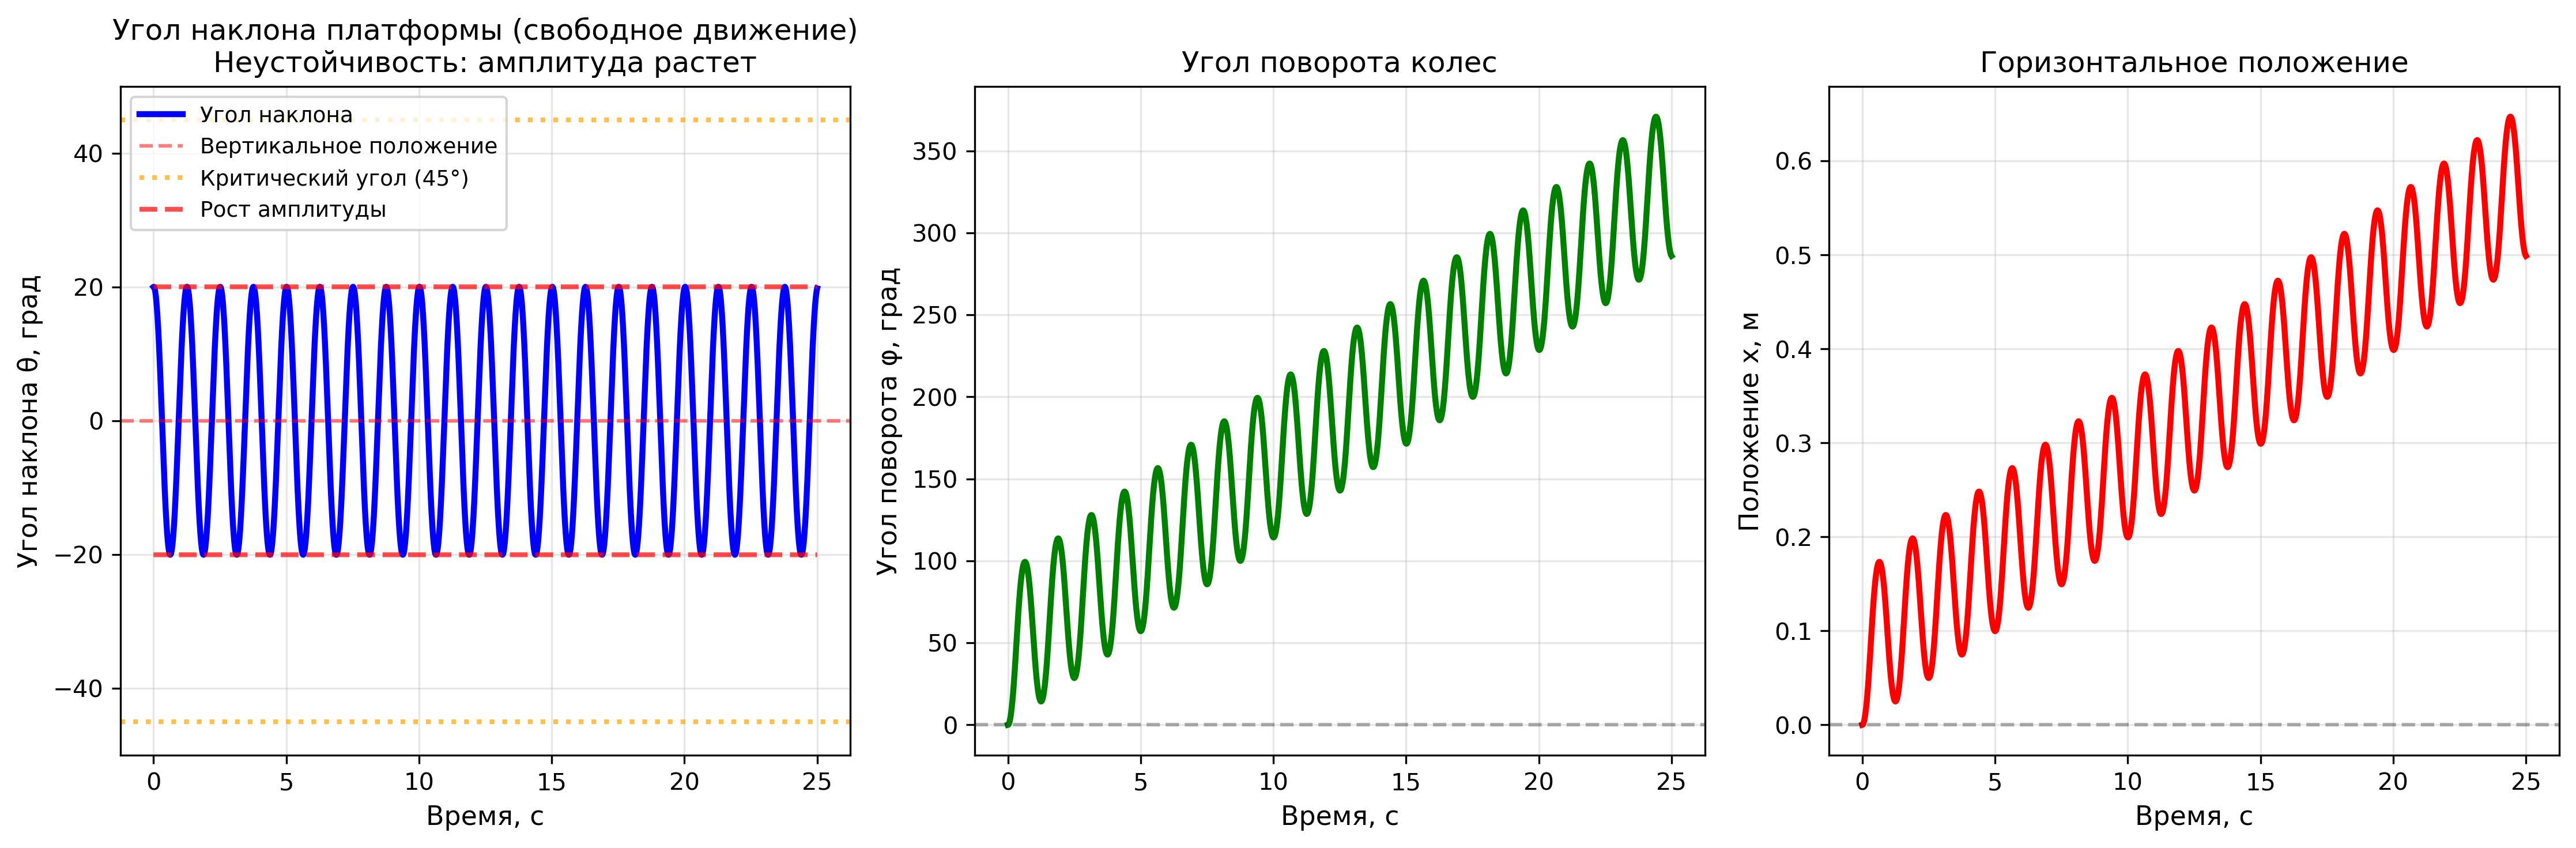
\includegraphics[width=0.75\textwidth,height=0.6\textheight,keepaspectratio]{images/free_motion.png}
\end{center}

\begin{block}{Выводы}
\begin{itemize}
    \item Система неустойчива в открытом контуре
    \item Малое отклонение приводит к падению
    \item Необходимо управление для стабилизации
\end{itemize}
\end{block}
\end{frame}


\section{Синтез системы управления}

\begin{frame}
\frametitle{Построение замкнутой системы}
\begin{block}{Замкнутая система}
\[
\mathbf{M}(\theta) \begin{bmatrix} \ddot{\theta} \\ \ddot{\phi} \end{bmatrix} + \mathbf{C} + \mathbf{G} = \begin{bmatrix} -K_p \theta - K_d \dot{\theta} \\ K_p \theta + K_d \dot{\theta} \end{bmatrix}
\]
\end{block}

\begin{block}{Параметры контроллера}
\begin{itemize}
    \item $K_p = 50.0$ --- пропорциональный коэффициент
    \item $K_d = 10.0$ --- дифференциальный коэффициент
\end{itemize}
\end{block}

\begin{block}{Критерии выбора}
\begin{itemize}
    \item Обеспечение устойчивости
    \item Минимизация времени установления
    \item Ограничение управления
\end{itemize}
\end{block}
\end{frame}

\section{Моделирование управляемого движения}

\begin{frame}
\frametitle{Результаты моделирования}
\begin{center}
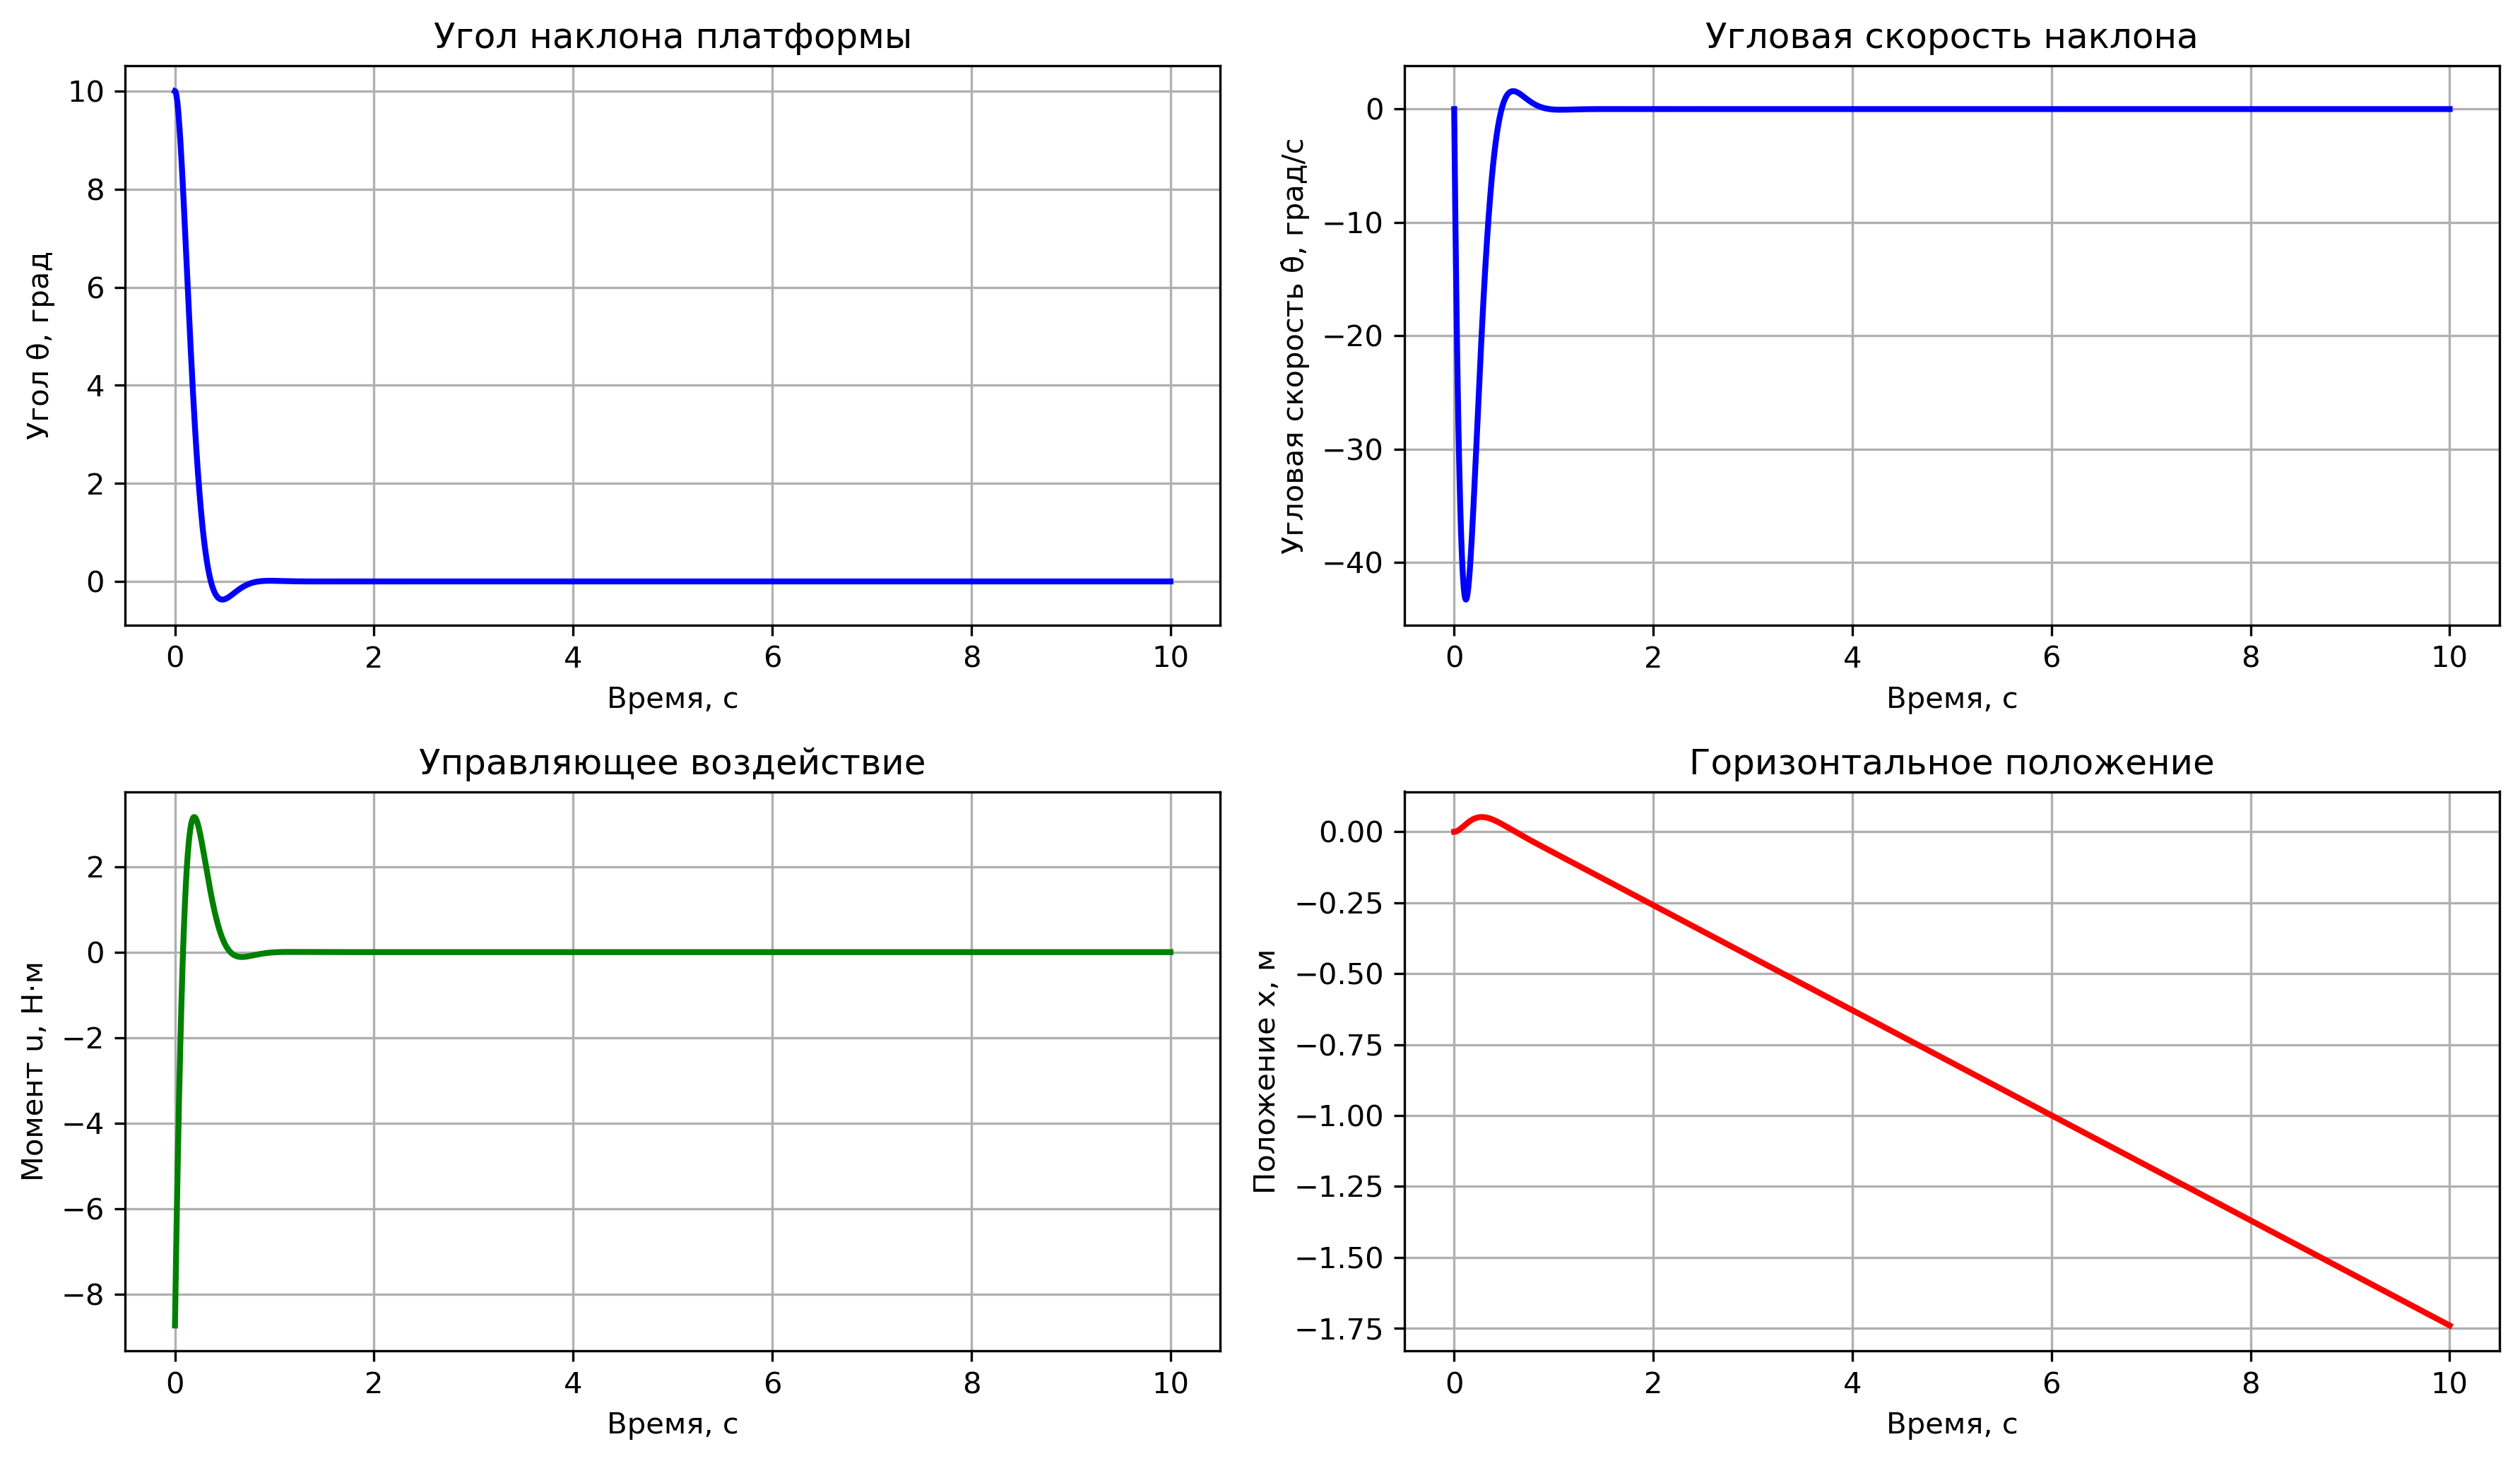
\includegraphics[width=0.75\textwidth,height=0.6\textheight,keepaspectratio]{images/controlled_motion_presentation.png}
\end{center}

\begin{block}{Характеристики}
\begin{itemize}
    \item Установившаяся ошибка: $< 0.000001°$
    \item Время установления: $0.283$ с
    \item Максимальный момент: $8.73$ Н·м
\end{itemize}
\end{block}
\end{frame}

\begin{frame}
\frametitle{Сравнение свободного и управляемого движения}
\begin{center}
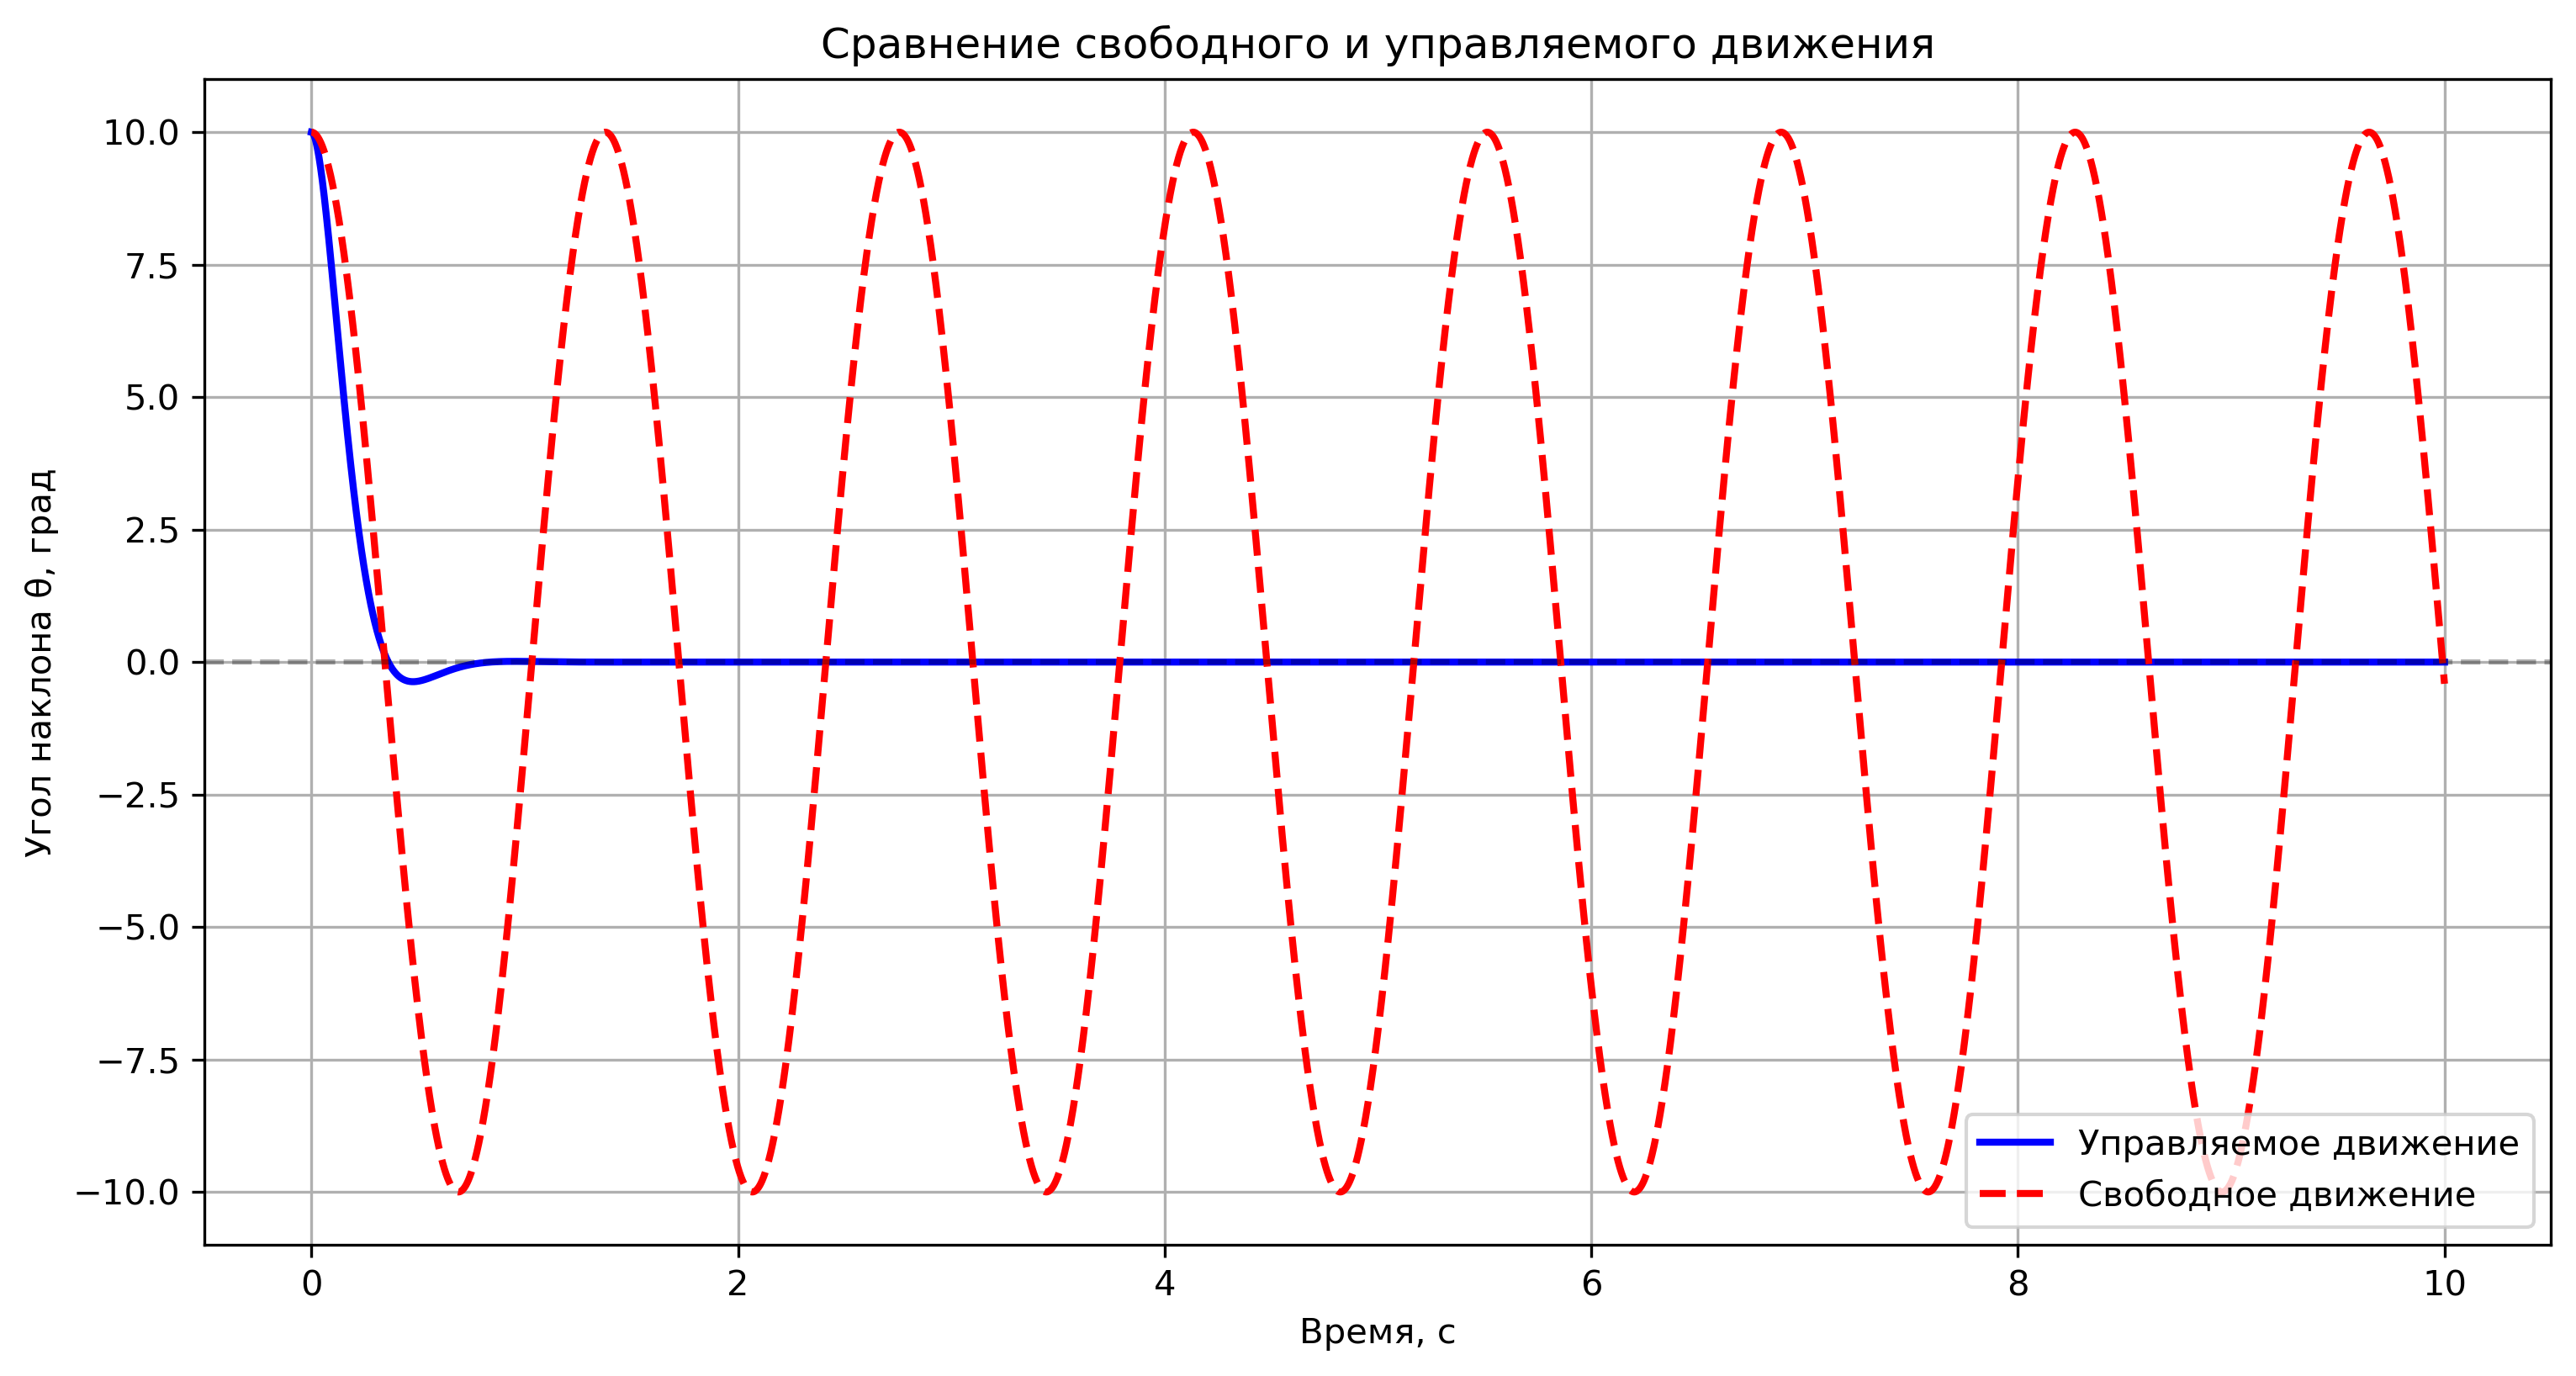
\includegraphics[width=0.75\textwidth,height=0.6\textheight,keepaspectratio]{images/comparison_free_vs_controlled.png}
\end{center}

Контроллер успешно стабилизирует систему
\end{frame}

\section{Анализ качества системы}

\begin{frame}
\frametitle{Оценка качества}
\begin{columns}
\column{0.5\textwidth}
\begin{block}{Устойчивость}
\begin{itemize}
    \item Асимптотическая устойчивость
    \item Экспоненциальная сходимость
    \item Все траектории сходятся к нулю
\end{itemize}
\end{block}

\column{0.5\textwidth}
\begin{block}{Точность}
\begin{itemize}
    \item Установившаяся ошибка: $< 0.000001°$
    \item Практически идеальная стабилизация
\end{itemize}
\end{block}
\end{columns}

\begin{block}{Быстродействие}
Время установления до $1°$: $0.283$ с
\end{block}
\end{frame}

\section{Заключение}



\begin{frame}
\frametitle{Выводы}
\begin{block}{Эффективность метода}
Метод управления по выходу успешно решает задачу стабилизации неполноприводной системы Segway
\end{block}

\begin{block}{Практическая применимость}
\begin{itemize}
    \item Использует только измеряемые переменные
    \item Простота реализации
    \item Высокое качество стабилизации
    \item Низкое энергопотребление
\end{itemize}
\end{block}
\end{frame}

\begin{frame}
\frametitle{}
\begin{center}
\Large Спасибо за внимание!
\end{center}
\end{frame}

\end{document}

